\documentclass[a4paper,11pt]{jsarticle}


% 数式
\usepackage{amsmath,amsfonts}
\usepackage{bm}
\usepackage{physics}
% 画像
\usepackage{graphicx}
\usepackage[dvipdfmx]{color}
% tikz関連
\usepackage{tikz}
\usetikzlibrary{intersections, calc, arrows.meta}
\usepackage{subcaption}


\begin{document}

\title{2次元有限要素法}
\author{伊東秀晃}
\date{\today}
\maketitle

\section*{1次三角形要素内の補間関数の適用/共役勾配法の実装}
以下の実装を行った。
\begin{enumerate}
  \item 1次三角形要素内の補間関数の適用
  \item \(\vb*{A^{*}}\vb*{u^{*}}=\vb*{f^{*}}\)のソルバとして共役勾配法を実装
\end{enumerate}
なお、1については1次三角形要素内の補間関数の適用をし、領域内の\(55\times55=3025\)の格子点に対して近似値を計算した。
2については、残差ベクトルの大きさの許容値は1e-5として計算した。

次に計算結果を可視化した図を示す。

\begin{figure}[htbp]
  \label{heatmap}
  \begin{tabular}{cc}
  \begin{minipage}[b]{0.45\linewidth}
    \centering
    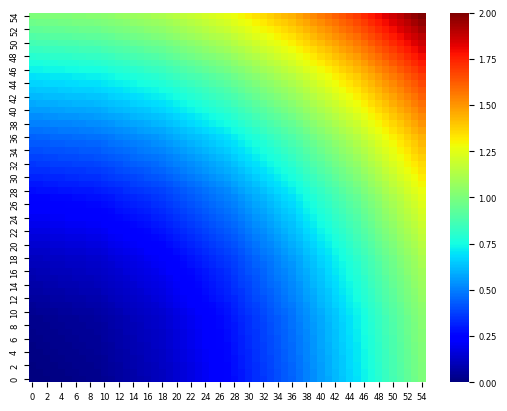
\includegraphics[keepaspectratio, scale=0.5]{img/gauss_72m.png}
    \subcaption{ガウス消去法による計算結果}
  \end{minipage} &
  \begin{minipage}[b]{0.45\linewidth}
    \centering
    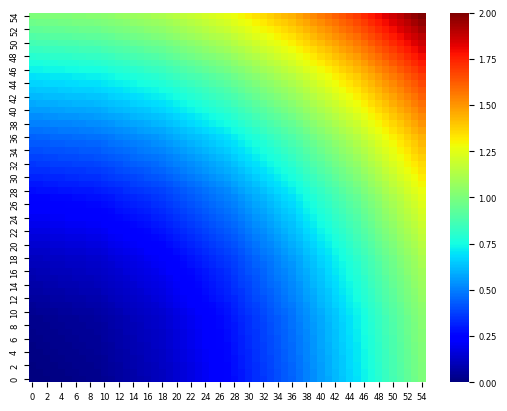
\includegraphics[keepaspectratio, scale=0.5]{img/CG_72m.png}
    \subcaption{共役勾配法による計算結果}
  \end{minipage}
\end{tabular}
\caption{要素内の補間関数を適用した。各軸の値はそれぞれ、xy座標の55倍の値。}
\end{figure}


\end{document}